
%%% Local Variables:
%%% mode: latex
%%% TeX-master: t
%%% End:

\documentclass{beamer}

\usetheme{boxes}
\usepackage[utf8]{inputenc}
\usepackage{tikz}
\usetikzlibrary{calc,shapes.multipart,chains,arrows}

\begin{document}

\begin{frame}

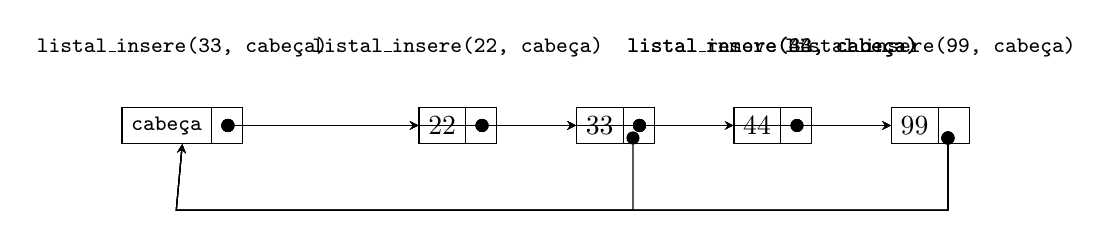
\begin{tikzpicture}
\def\shift{2cm}
\def\cabeca{{\tt cabe\c{c}a}}

\tikzset{
    list/.style={rectangle split, rectangle split parts=2,
    draw, rectangle split horizontal}, 
    >=stealth, start chain
}

  \node[list,on chain] (HEAD) {\footnotesize \cabeca};
  \node[] (BACKLINK) [below of=HEAD] {};

  \node[]  (FIRST) [right of=HEAD,xshift=.5*\shift]  {};
  \node[]  (SECOND) [right of=FIRST,xshift=.5*\shift] {};
  \node[]  (THIRD) [right of=SECOND,xshift=.5*\shift] {};
  \node[]  (FOURTH) [right of=THIRD,xshift=.5*\shift] {};
  \node<4-6>[list,on chain] (C) at (FIRST) {22};
  \node<2-5>[list,on chain] (A) at  (SECOND) {33};
  \node<3->[list,on chain]  (B) at (FOURTH) {99};
  \node<5->[list,on chain]  (D) at (THIRD) {44};
  
  %INSERE 33
  \node<2> [above of=HEAD] {{\tt\footnotesize listal\_insere(33, \cabeca)}};
  \draw<2>[*->] let \p1 = (HEAD.two), \p2 = (HEAD.center) in (\x1,\y2)  -- (A);
  \draw<2>[*->] (A.two) -- +(0,-.5*\shift) --
  +(-2.9*\shift,-.5*\shift) -- (HEAD.south);


  %INSERE 99
  \def\tail{B}
  \node<3> [above of=\tail] {{\tt\footnotesize listal\_insere(99, \cabeca)}};
  \draw<3>[*->] let \p1 = (HEAD.two), \p2 = (HEAD.center) in (\x1,\y2)  -- (A);
  \draw<3>[*->] let \p1 = (A.two), \p2 = (A.center) in (\x1,\y2) -- (B);
  \draw<3>[*->] (B.two) -- +(0,-.5*\shift) --
  +(-4.9*\shift,-.5*\shift) -- (HEAD.south);

  

  %INSERE 22
  \def\tail{C}
  \node<4> [above of=\tail] {{\tt\footnotesize listal\_insere(22, \cabeca)}};
  \draw<4>[*->] let \p1 = (HEAD.two), \p2 = (HEAD.center) in (\x1,\y2)  -- (C);
  \draw<4>[*->] let \p1 = (C.two), \p2 = (C.center) in (\x1,\y2) -- (A);
  \draw<4>[*->] let \p1 = (A.two), \p2 = (A.center) in (\x1,\y2)  -- (B);
  \draw<4>[*->] (B.two) -- +(0,-.5*\shift) --
  +(-4.9*\shift,-.5*\shift) -- (HEAD.south);



  %INSERE 44
   \def\tail{D}
   \node<5> [above of=\tail] {{\tt\footnotesize listal\_insere(44, \cabeca)}};
   \draw<5>[*->] let \p1 = (HEAD.two), \p2 = (HEAD.center) in (\x1,\y2)  -- (C);
   \draw<5>[*->] let \p1 = (C.two), \p2 = (C.center) in (\x1,\y2) -- (A);
   \draw<5>[*->] let \p1 = (A.two), \p2 = (A.center) in (\x1,\y2) -- (D);
   \draw<5>[*->] let \p1 = (D.two), \p2 = (D.center) in (\x1,\y2)  -- (B);
   \draw<5>[*->] (B.two) -- +(0,-.5*\shift) --
   +(-4.9*\shift,-.5*\shift) -- (HEAD.south);


  %REMOVE 33
  \def\tail{D}
  \node<6> [above of=\tail] {{\tt\footnotesize listal\_remove(33, \cabeca)}};
   \draw<6>[*->] let \p1 = (HEAD.two), \p2 = (HEAD.center) in (\x1,\y2)  -- (C);
   \draw<6>[*->] let \p1 = (C.two), \p2 = (C.center) in (\x1,\y2) -- (D);
   \draw<6>[*->] let \p1 = (D.two), \p2 = (D.center) in (\x1,\y2)  -- (B);
   \draw<6>[*->] (B.two) -- +(0,-.5*\shift) --
   +(-4.9*\shift,-.5*\shift) -- (HEAD.south);

\end{tikzpicture}

\end{frame}

\end{document}